\chapter{Appendix about the axion peaks}
\label{ch:alp_appendix}

\section{Further discussion}
% \mnote{In this paragraph discuss the the distribution of the p-values and plot the filtered p-values.}
% \mnote{Now, proceed to discuss the distribution of p-values. Then, proceed to plot the filtered p-values as the function of frequency.}
There were a number of frequencies where statistically significant excesses were observed in the datasets sensitive to an oscillating nEDM.
Even though the excesses are not compatible with an axion-induced signal, it is interesting to investigate the possible reason.

In the first step we look at the p-value distribution, shown in black in Fig.\,\ref{fig:axions_P_p-values} (for the EB parallel dataset).
The distribution is flat with narrow peak in the first bin, corresponding to the highest excesses.
This means that there is only a small number (around 300 out of \num[detect-all=true]{156198}) frequencies, where more power than expected is observed.
\marginpar{A global, like over- or underestimating the error-bars, would cause a tilt in the p-value distribution.}
To identify this group we plot the ratio of the observed to average amplitude (Fig.\,\ref{fig:axions_observed-predicted_power_ratio_filtered}). The lines are low-pass filtered to average the statistical noise out. The excesses occur only for frequencies below \SI{1e-4}{\hertz} and in a narrow region around inverse \SI{300}{\second}. These are the regions where the gradient-drift correction had an effect.

Here tell how it might be due to the imperfect gradient-drift correction. Say, that the narrow region around inverse \SI{300}{\second} is most likely strongly correlated with the low frequencies (essentially peak folding around the Nyquist frequency in the case of evenly sampled data.)


\begin{figure}
  \centering
  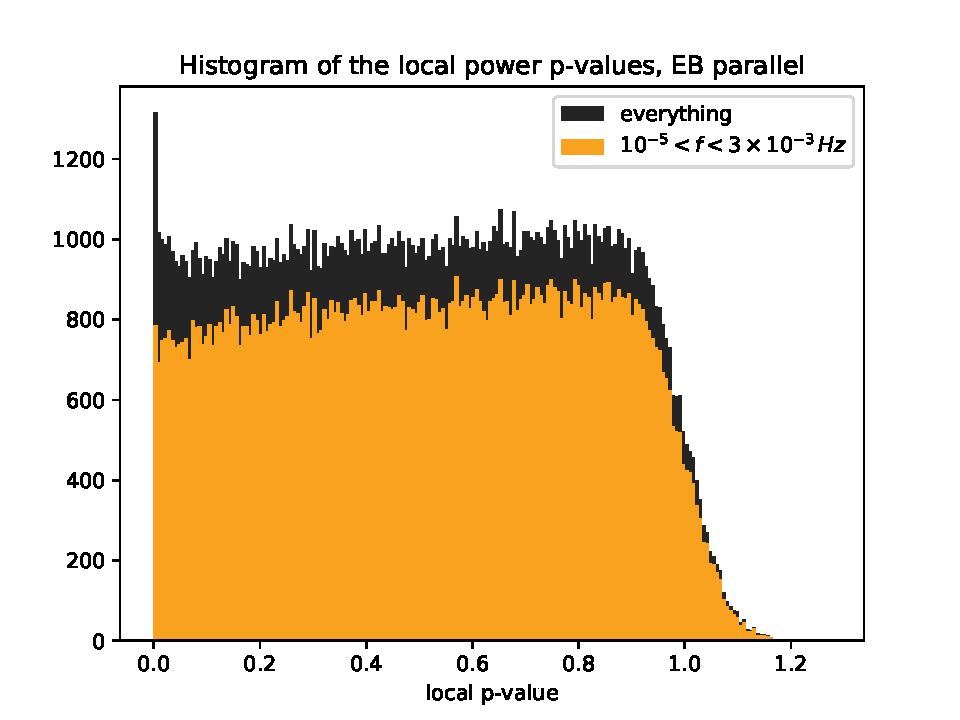
\includegraphics[width=0.9\linewidth]{gfx/axions/P_p-values.pdf}
  \caption{Accounting for the look-elsewhere effect for the parallel dataset. It provides the minimal local p-value -- global p-value transition. The fit with the model \dots gives the number of frequencies. \note{Prepare this histogram in a way, that the curves for all the datasets are shown. Then may need to normalise it.}}
  \label{fig:axions_P_p-values}
\end{figure}

\begin{figure}
  \centering
  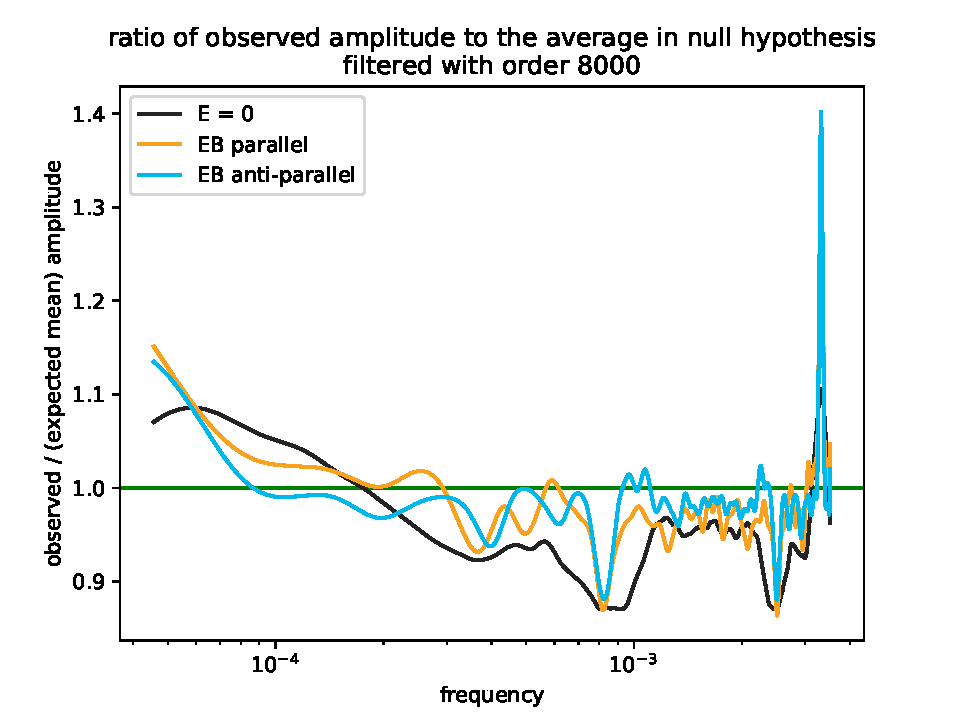
\includegraphics[width=0.9\linewidth]{gfx/axions/observed-predicted_power_ratio_filtered.pdf}
  \caption{Maybe mark the 1/300 seconds. Note, that because of the settling of the filter first $N$ points need to be dropped, so not whole range is plotted.}
  \label{fig:axions_observed-predicted_power_ratio_filtered}
\end{figure}



The idea is to give them all for completeness.
\mnote{Also, put the axion wind plots here!}



\section{EB anti-parallel}
\begin{figure}
  \centering
  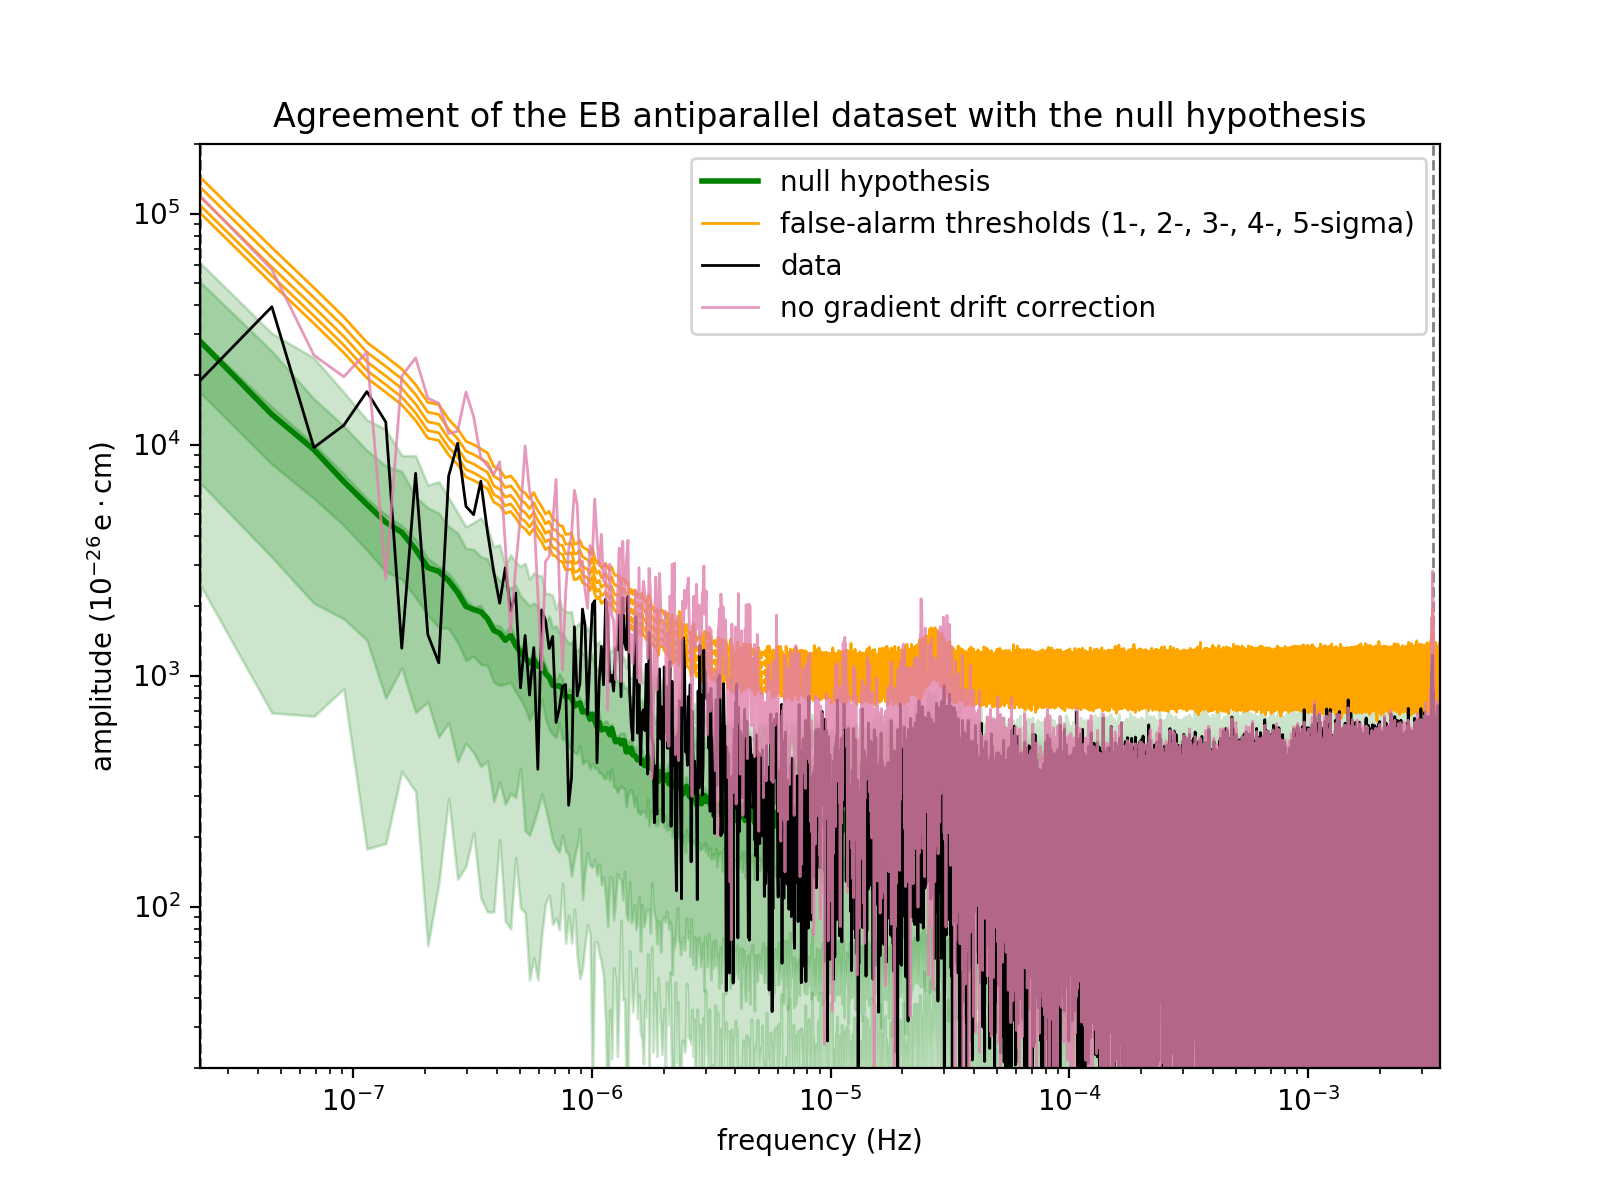
\includegraphics[width=\linewidth]{gfx/axions/AP_detection_and_no_GDC.png}
  \caption{\ldots}
  \label{fig:axions_AP_detection_and_no_GDC}
\end{figure}
\begin{figure}
  \centering
  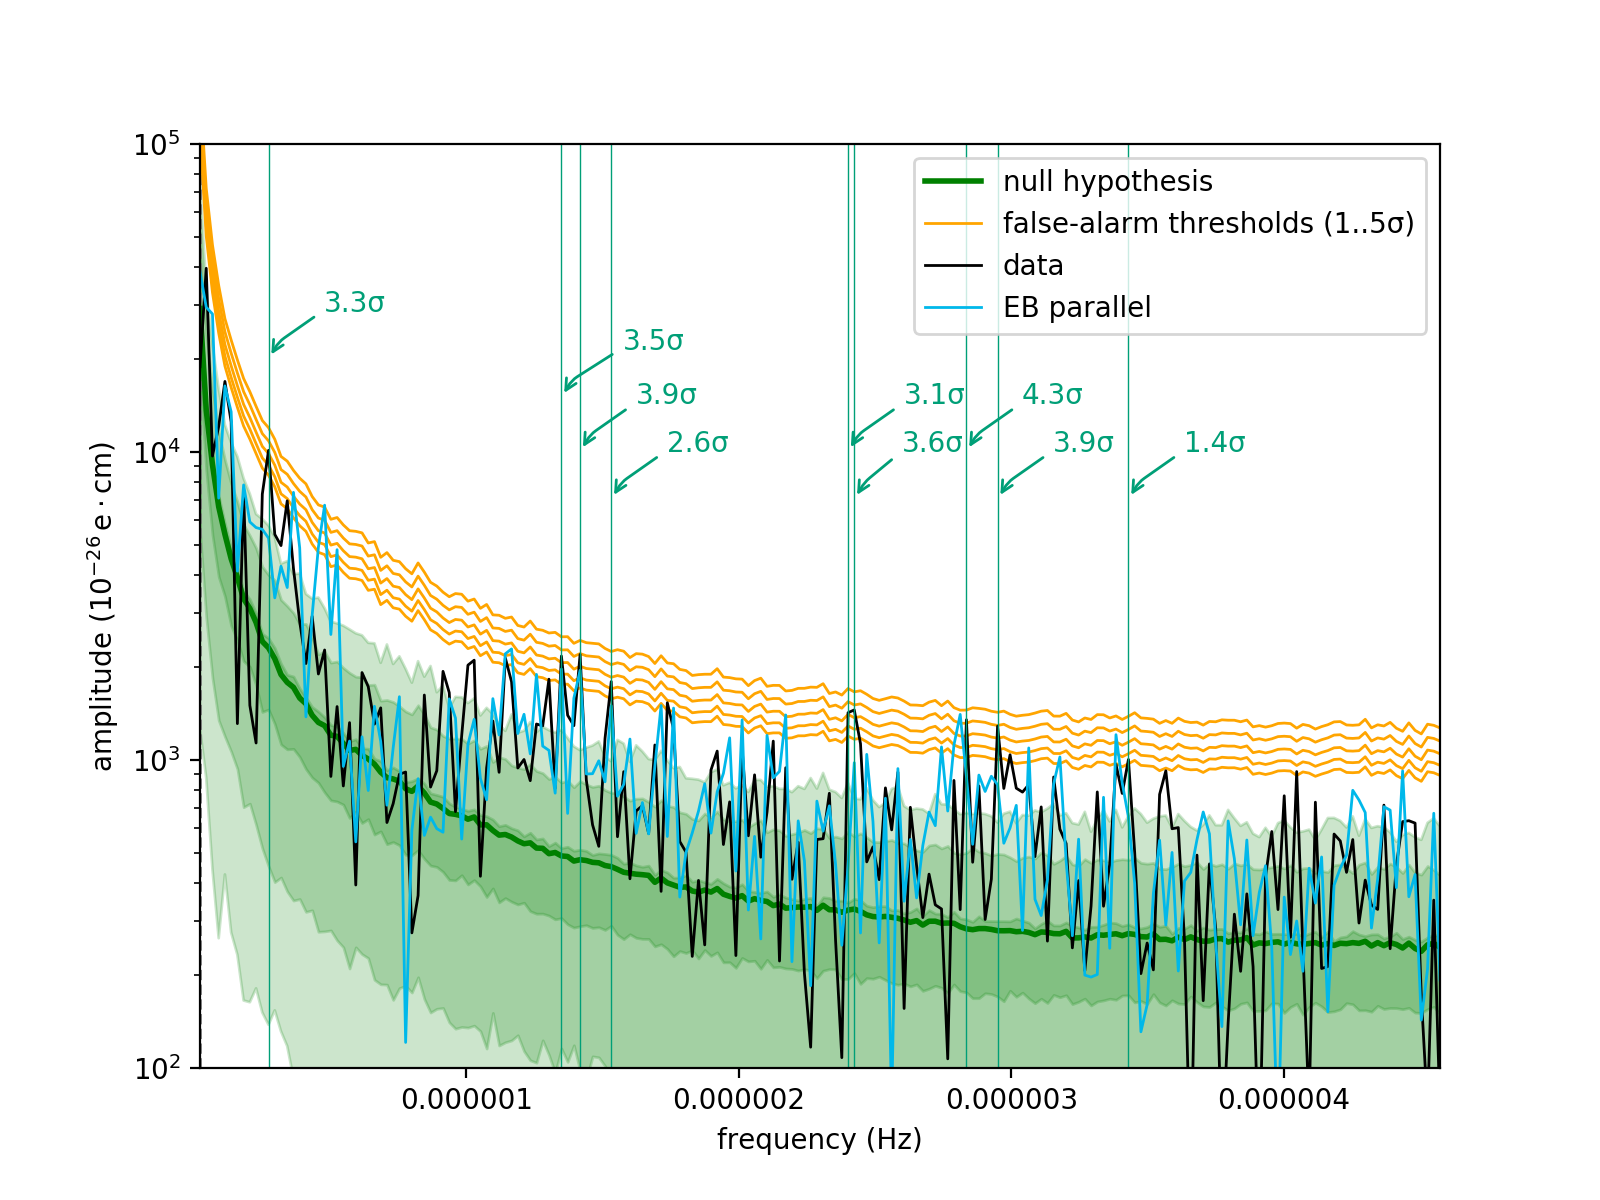
\includegraphics[width=\linewidth]{gfx/axions/AP_detection_area1.png}
  \caption{\ldots}
  \label{fig:axions_AP_detection_area1}
\end{figure}
\begin{figure}
  \centering
  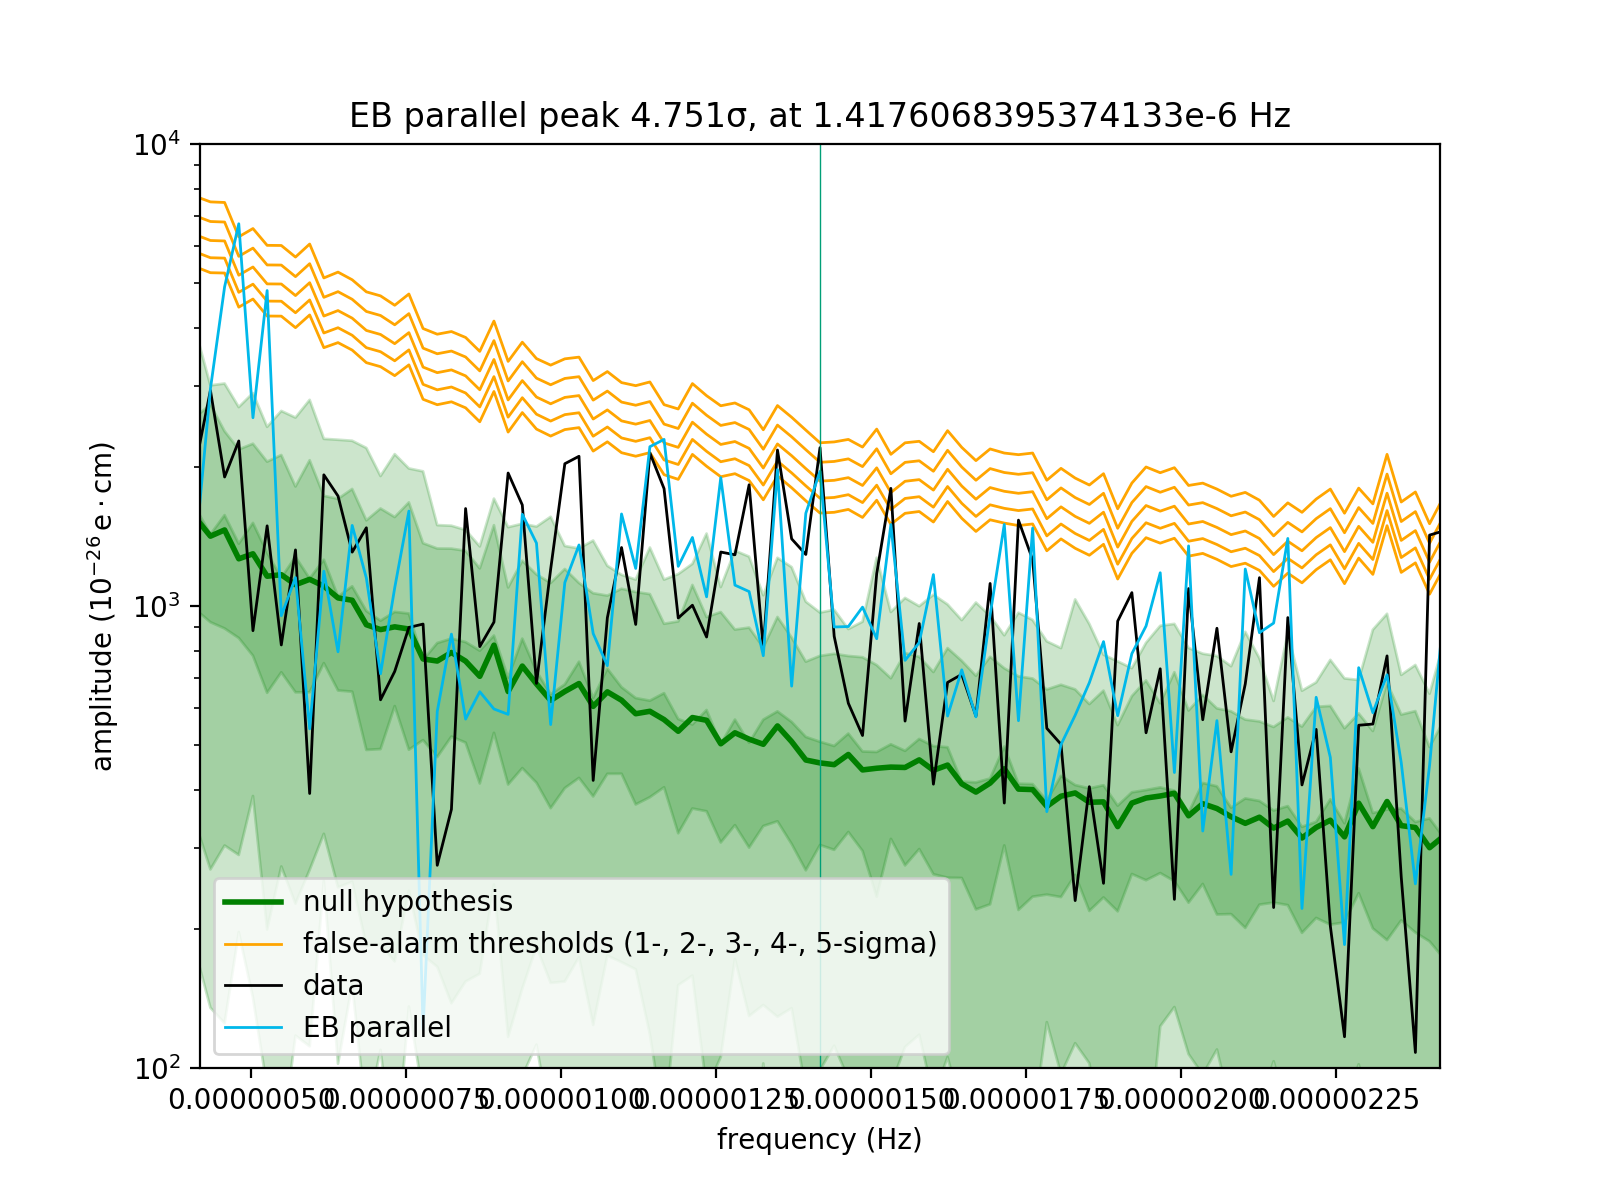
\includegraphics[width=\linewidth]{gfx/axions/AP_detection_peak_62.png}
  \caption{\ldots}
  \label{fig:AP_detection_peak_62}
\end{figure}
\begin{figure}
  \centering
  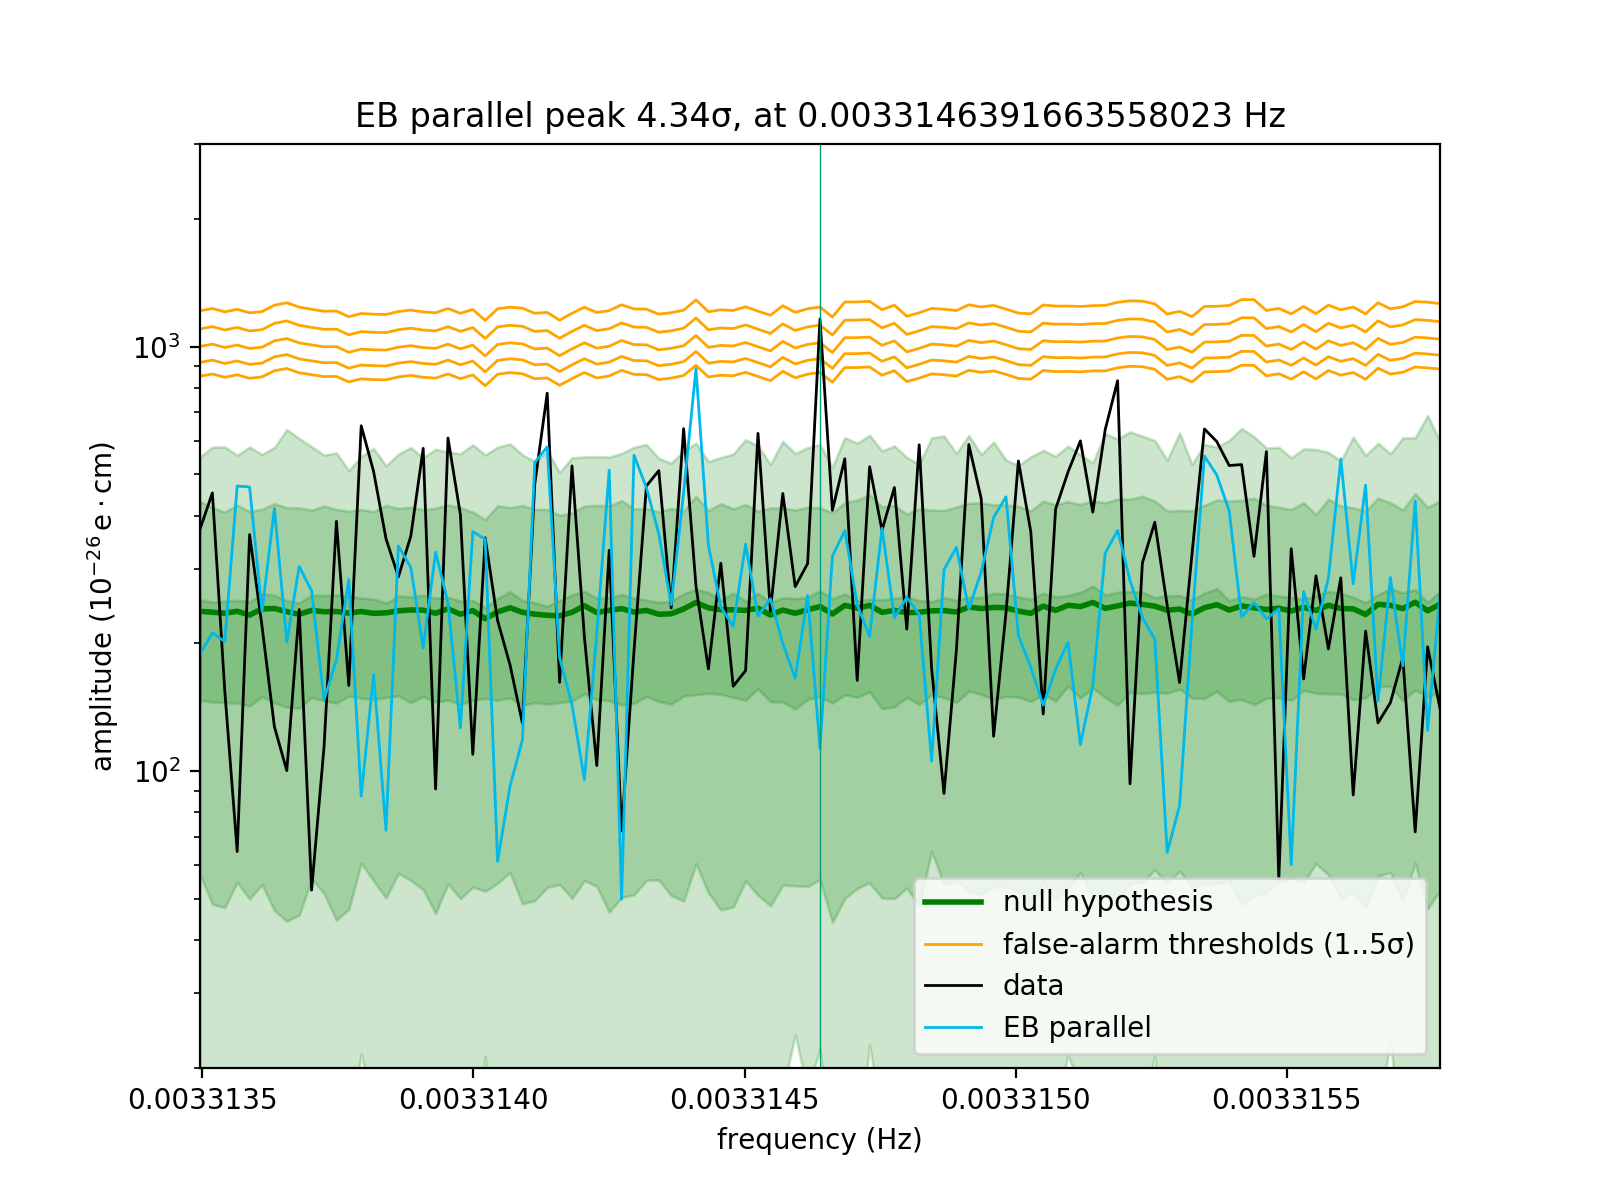
\includegraphics[width=\linewidth]{gfx/axions/AP_detection_peak_144968.png}
  \caption{\ldots}
  \label{fig:AP_detection_peak_144968}
\end{figure}


\section{EB parallel}

\begin{figure}
  \centering
  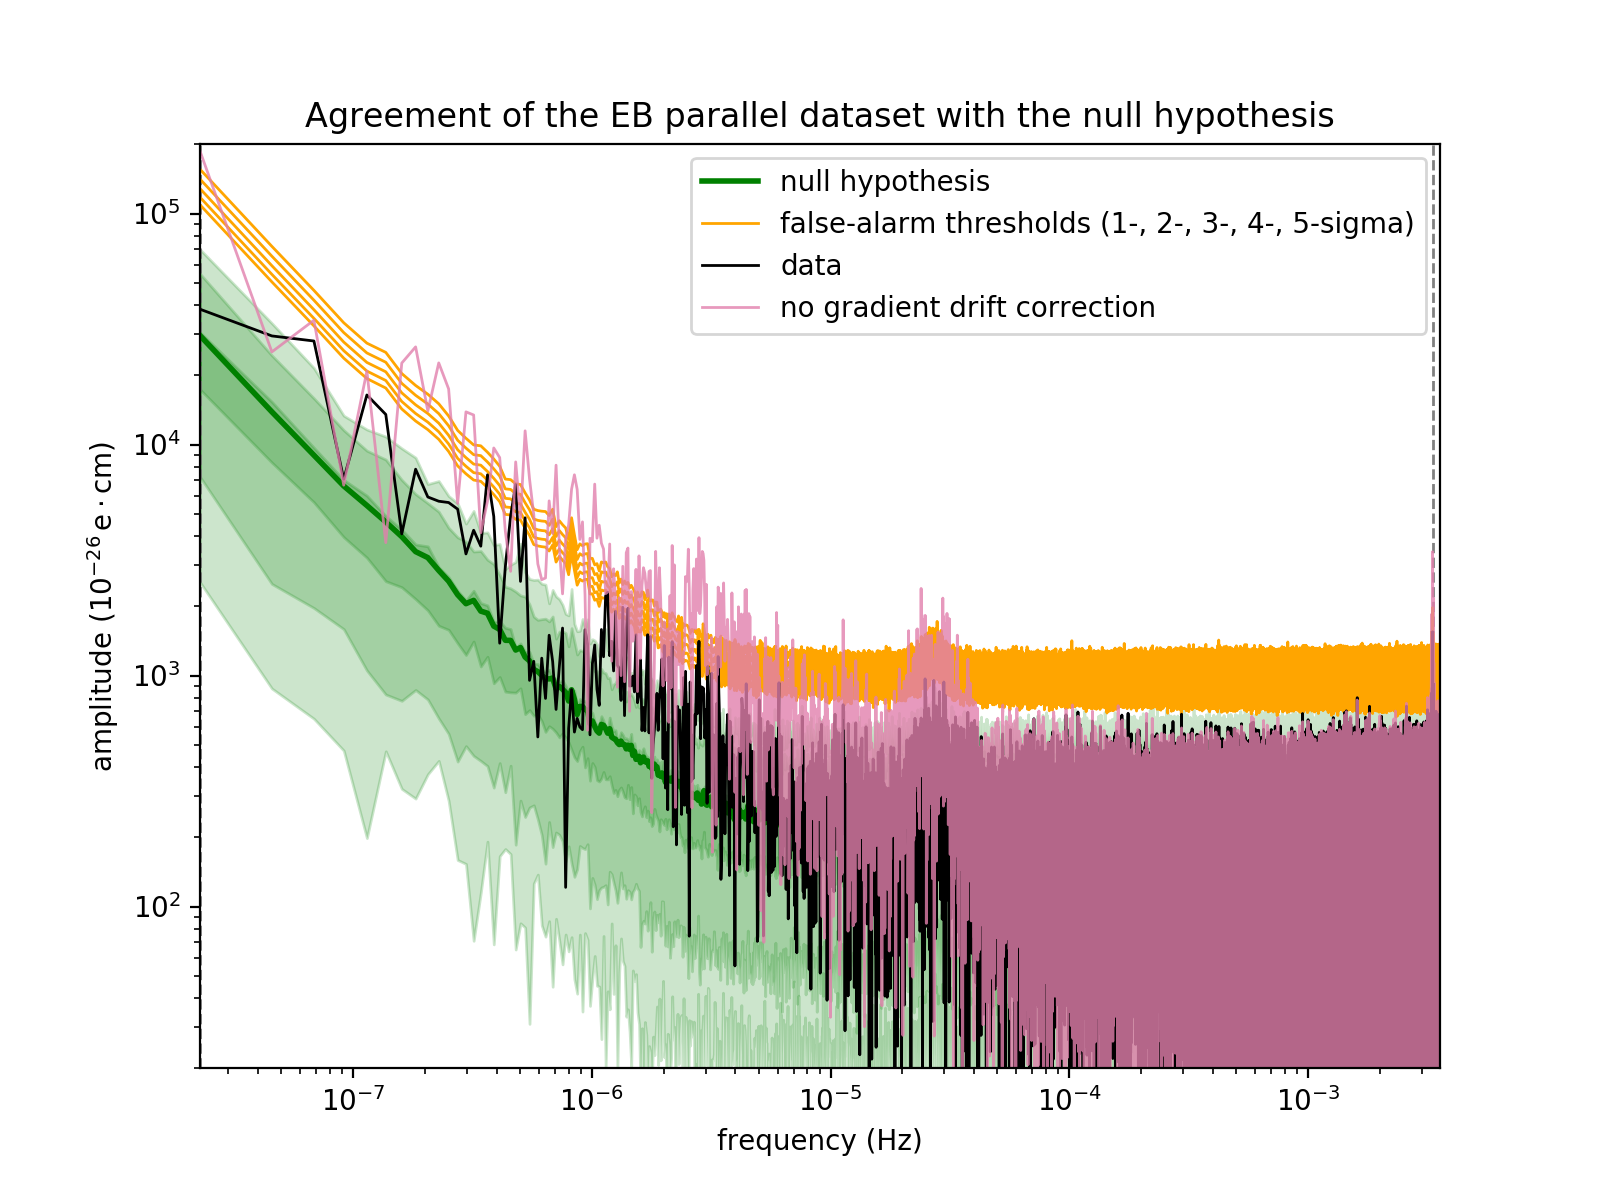
\includegraphics[width=\linewidth]{gfx/axions/P_detection_and_no_GDC.png}
  \caption{\ldots}
  \label{fig:P_detection_and_no_GDC}
\end{figure}
\begin{figure}
  \centering
  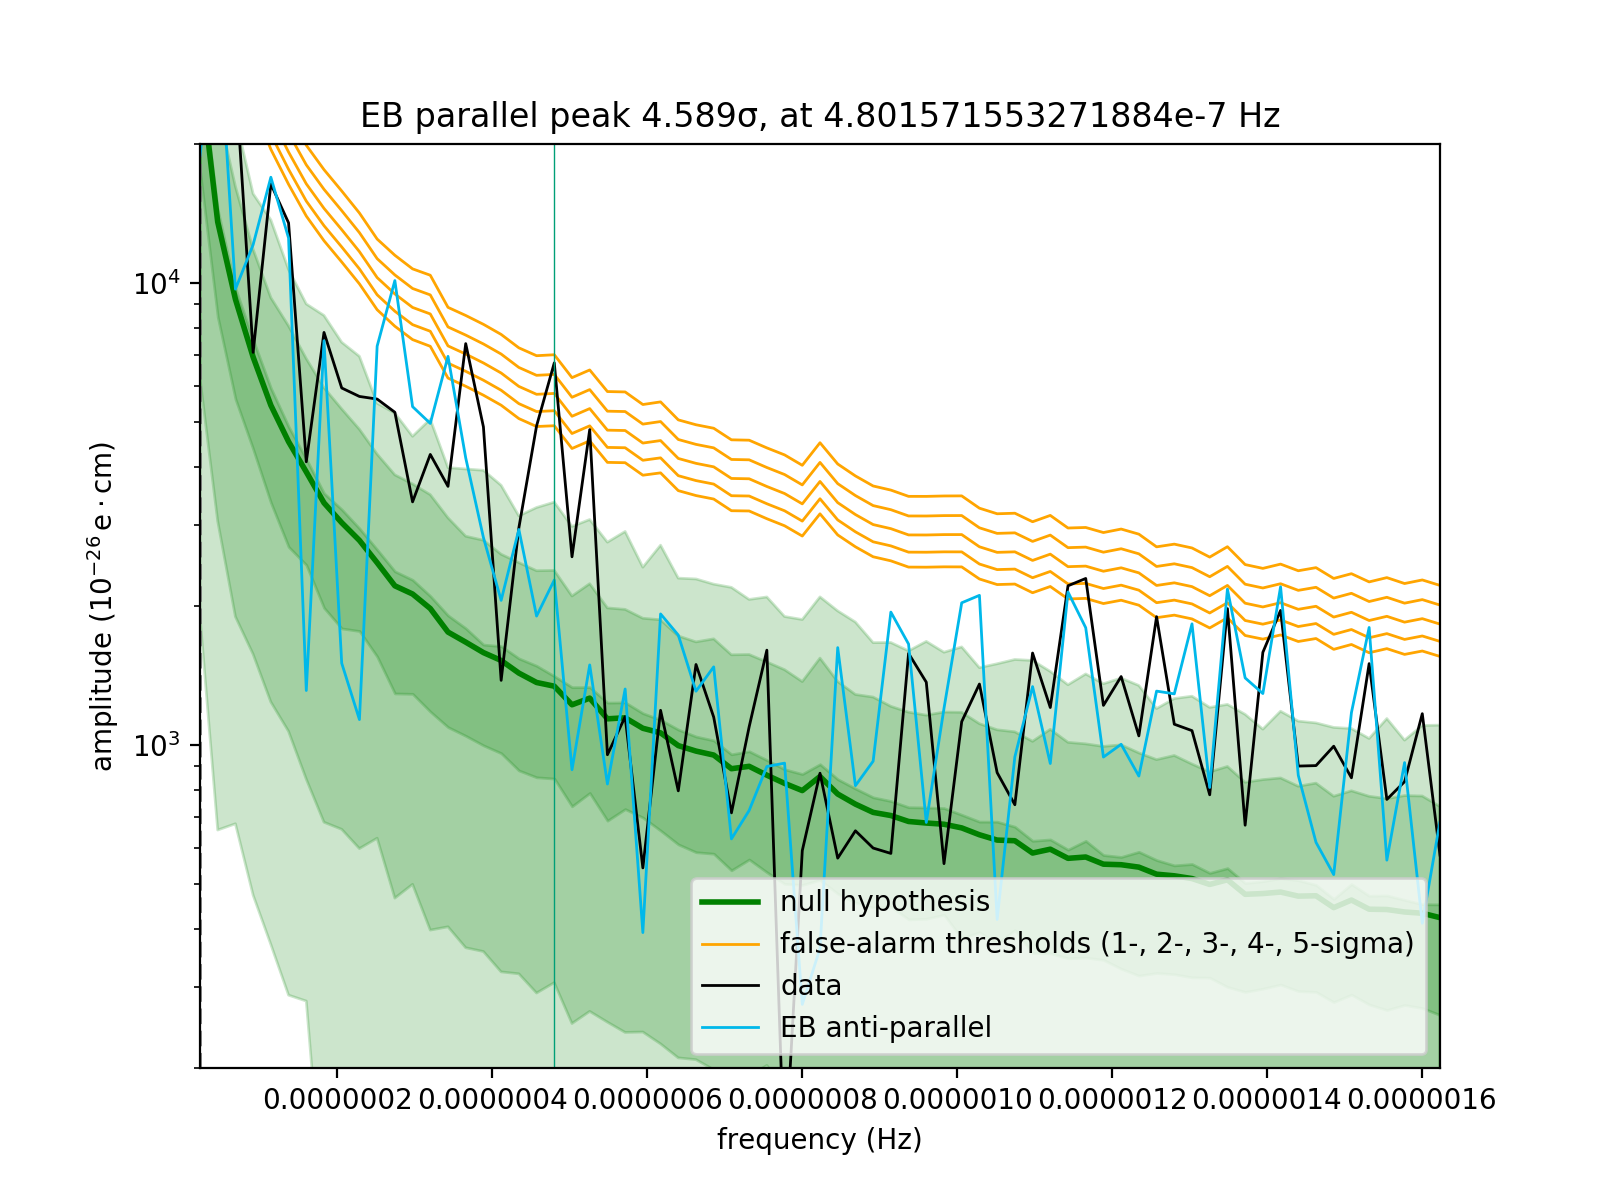
\includegraphics[width=\linewidth]{gfx/axions/P_detection_peak_21.png}
  \caption{\ldots}
  \label{fig:P_detection_peak_21}
\end{figure}
\begin{figure}
  \centering
  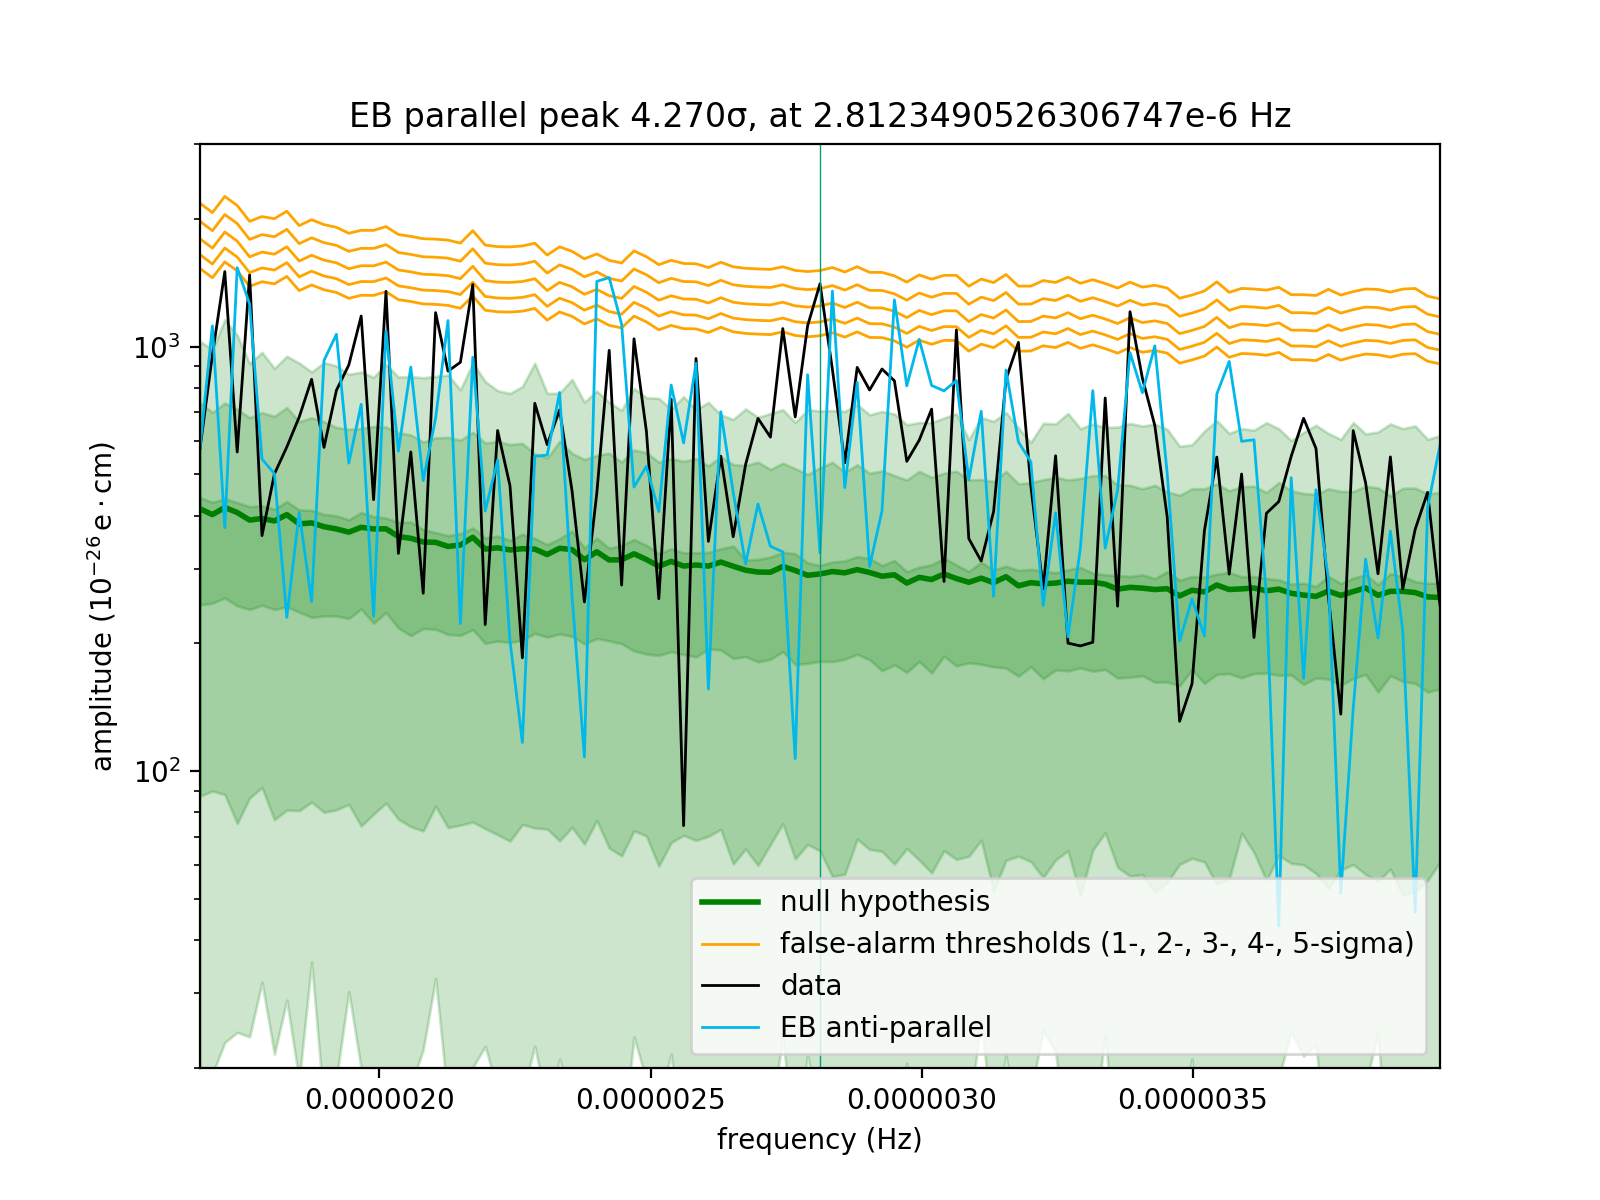
\includegraphics[width=\linewidth]{gfx/axions/P_detection_peak_123.png}
  \caption{\ldots}
  \label{fig:P_detection_peak_123}
\end{figure}
\begin{figure}
  \centering
  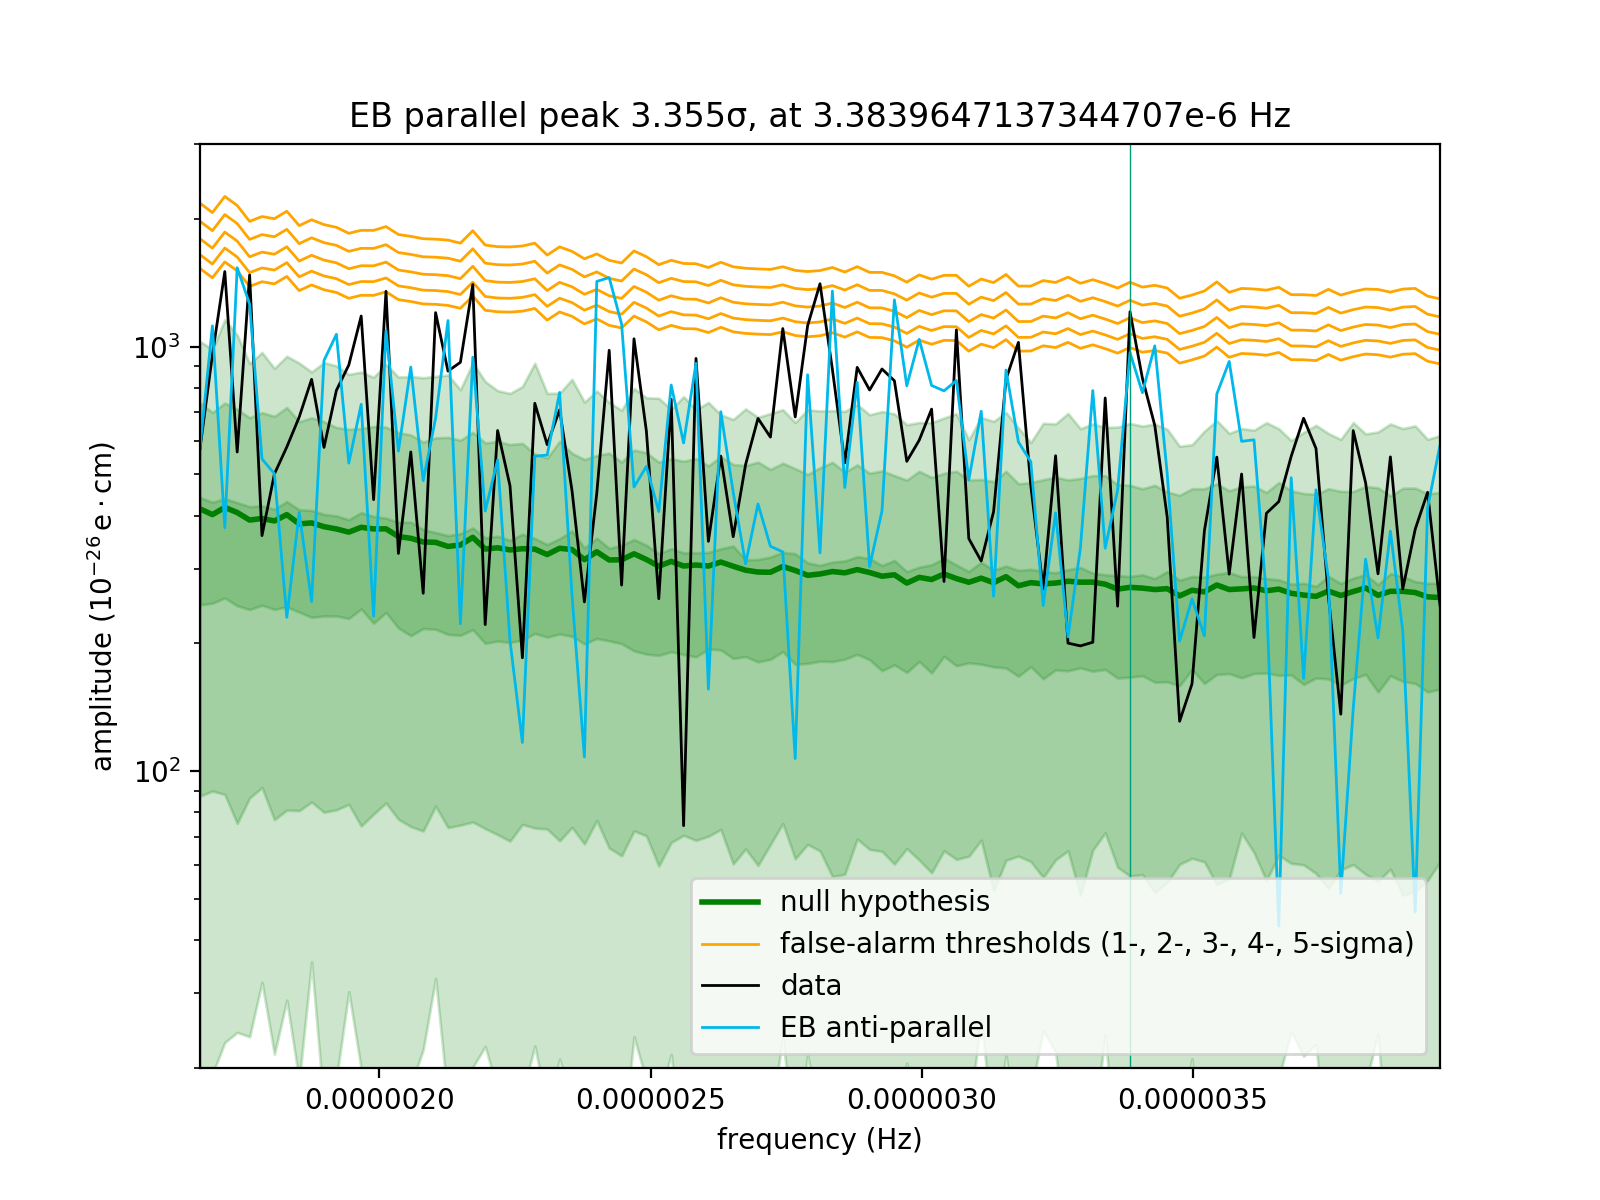
\includegraphics[width=\linewidth]{gfx/axions/P_detection_peak_148.png}
  \caption{\ldots}
  \label{fig:P_detection_peak_148}
\end{figure}
\begin{figure}
  \centering
  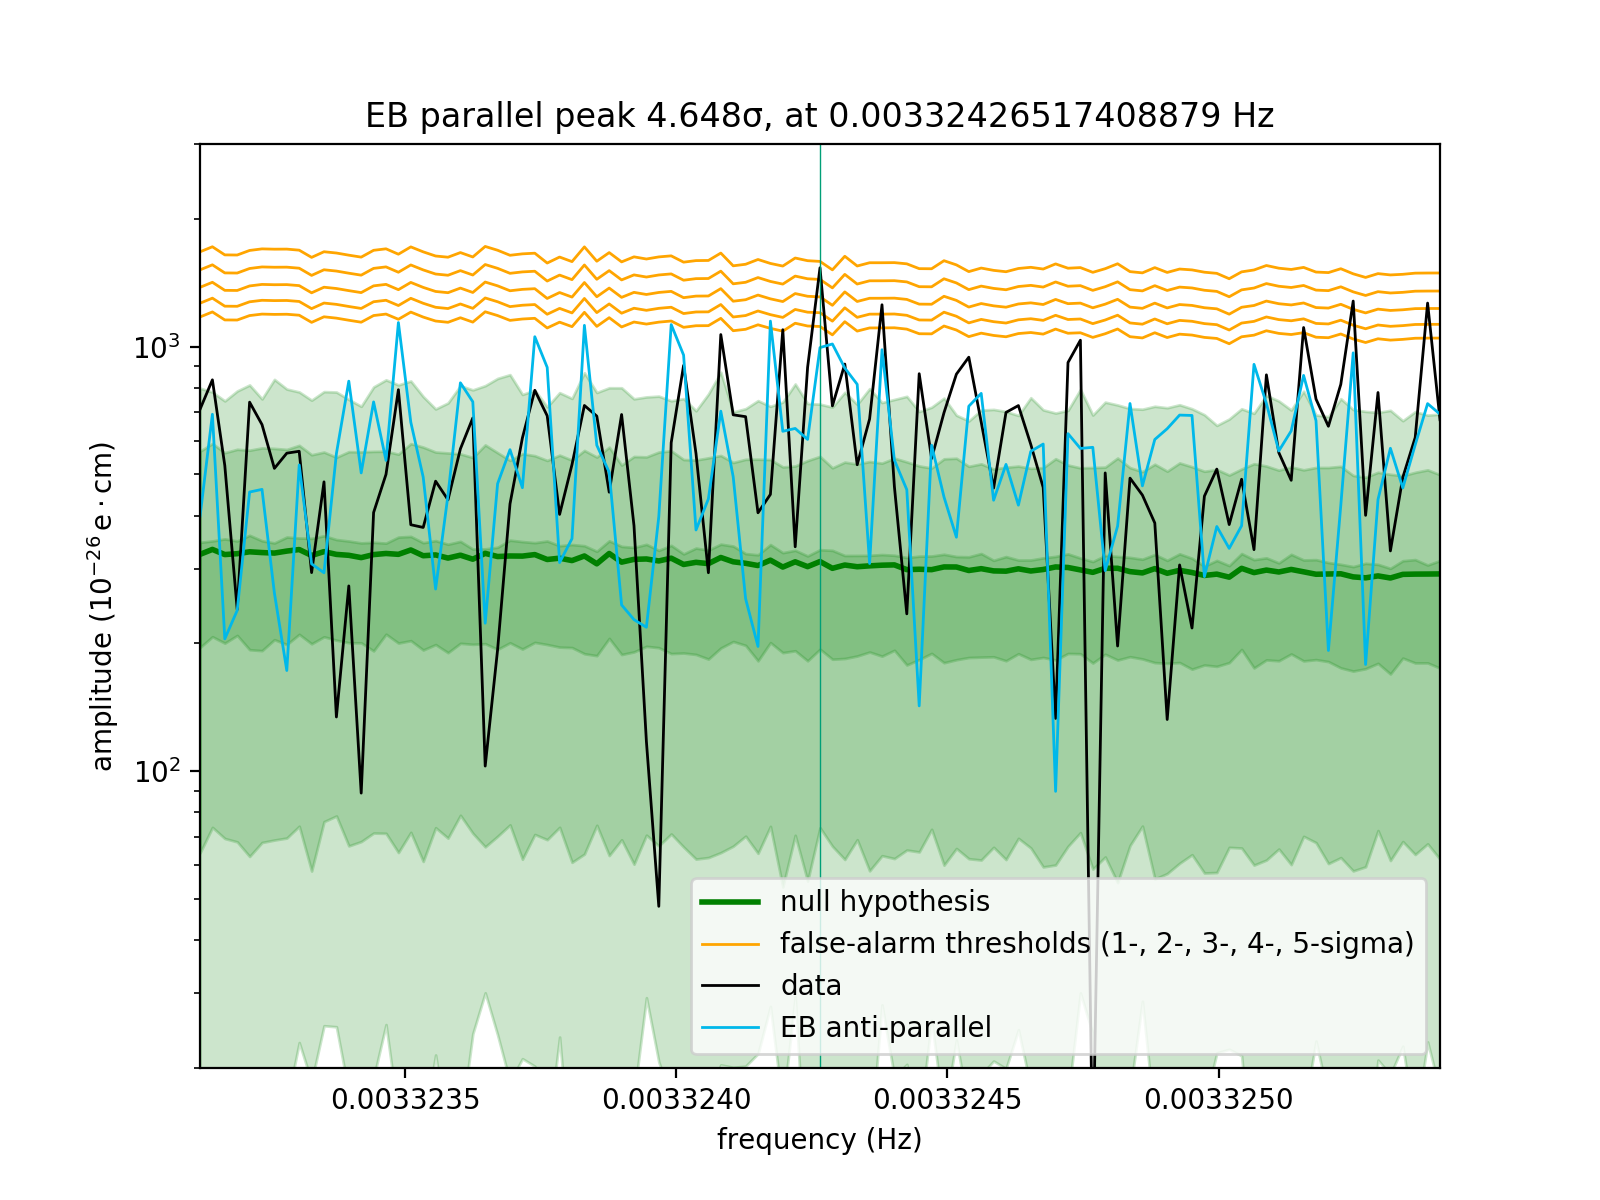
\includegraphics[width=\linewidth]{gfx/axions/P_detection_peak_145389.png}
  \caption{\ldots}
  \label{fig:P_detection_peak_145389}
\end{figure}
\begin{figure}
  \centering
  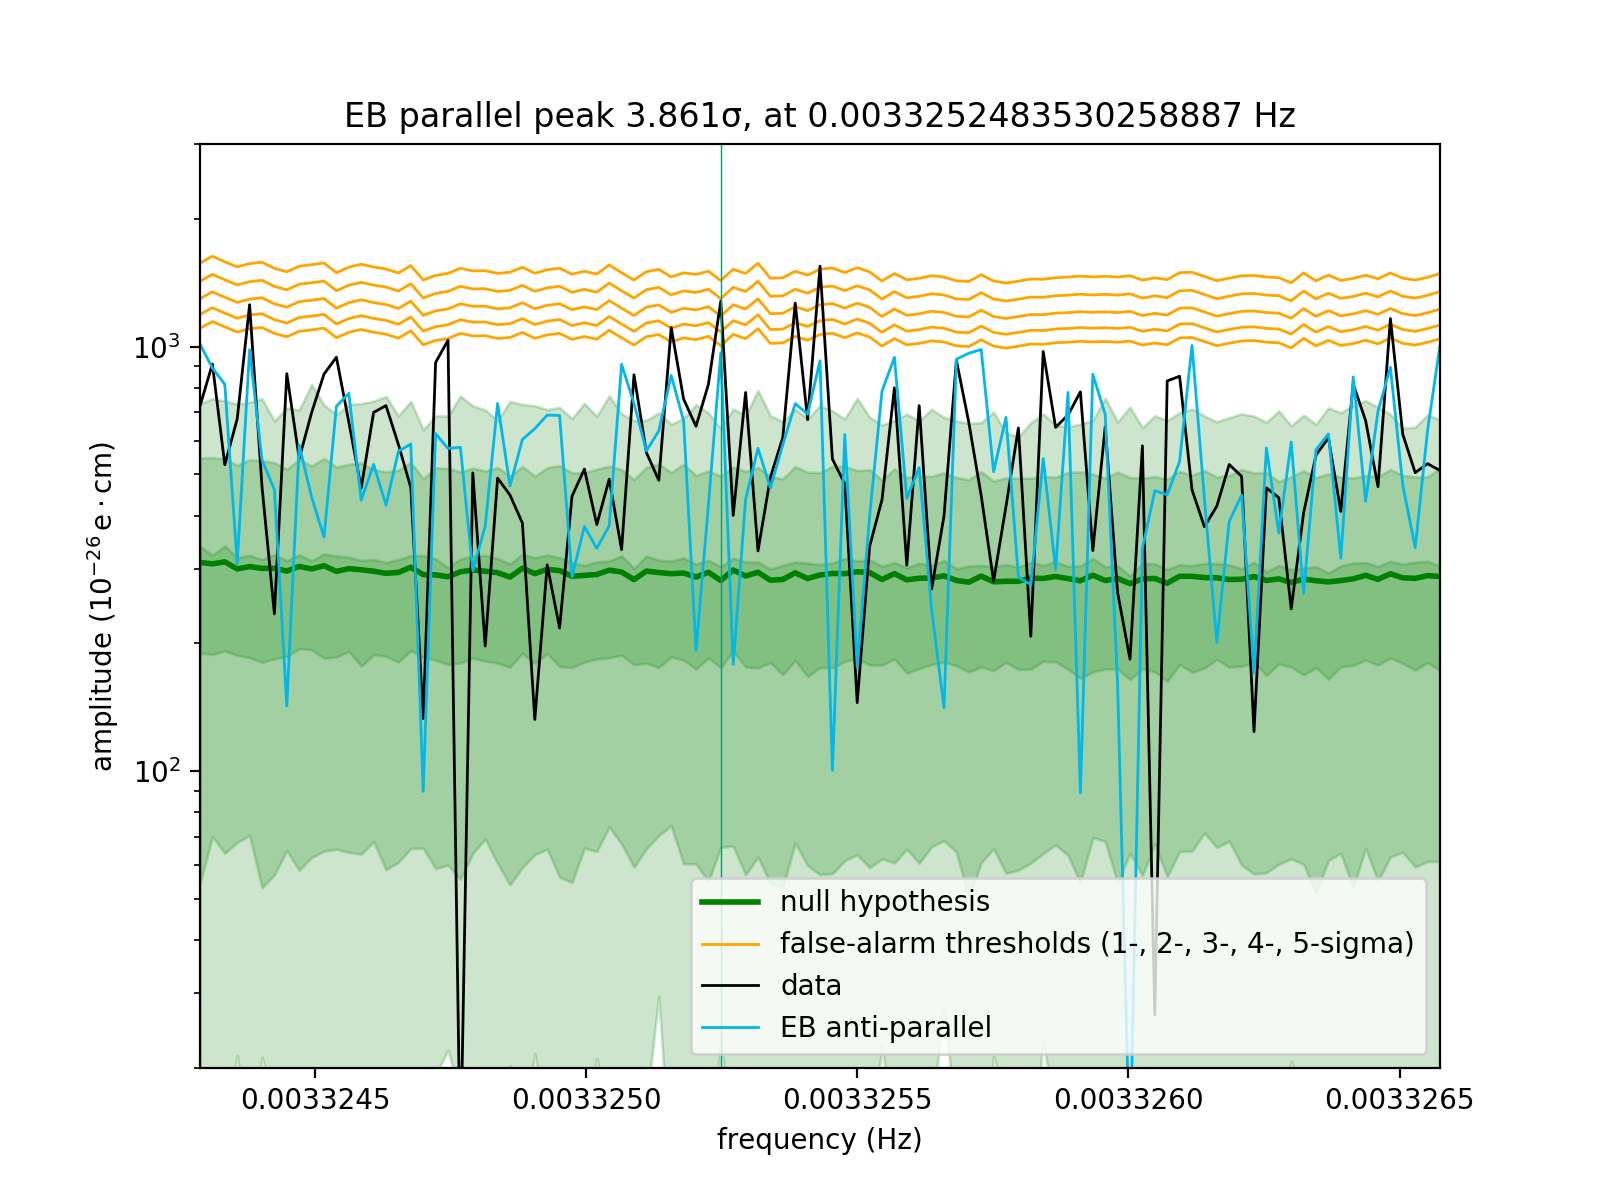
\includegraphics[width=\linewidth]{gfx/axions/P_detection_peak_145432.png}
  \caption{\ldots}
  \label{fig:P_detection_peak_145432}
\end{figure}
\begin{figure}
  \centering
  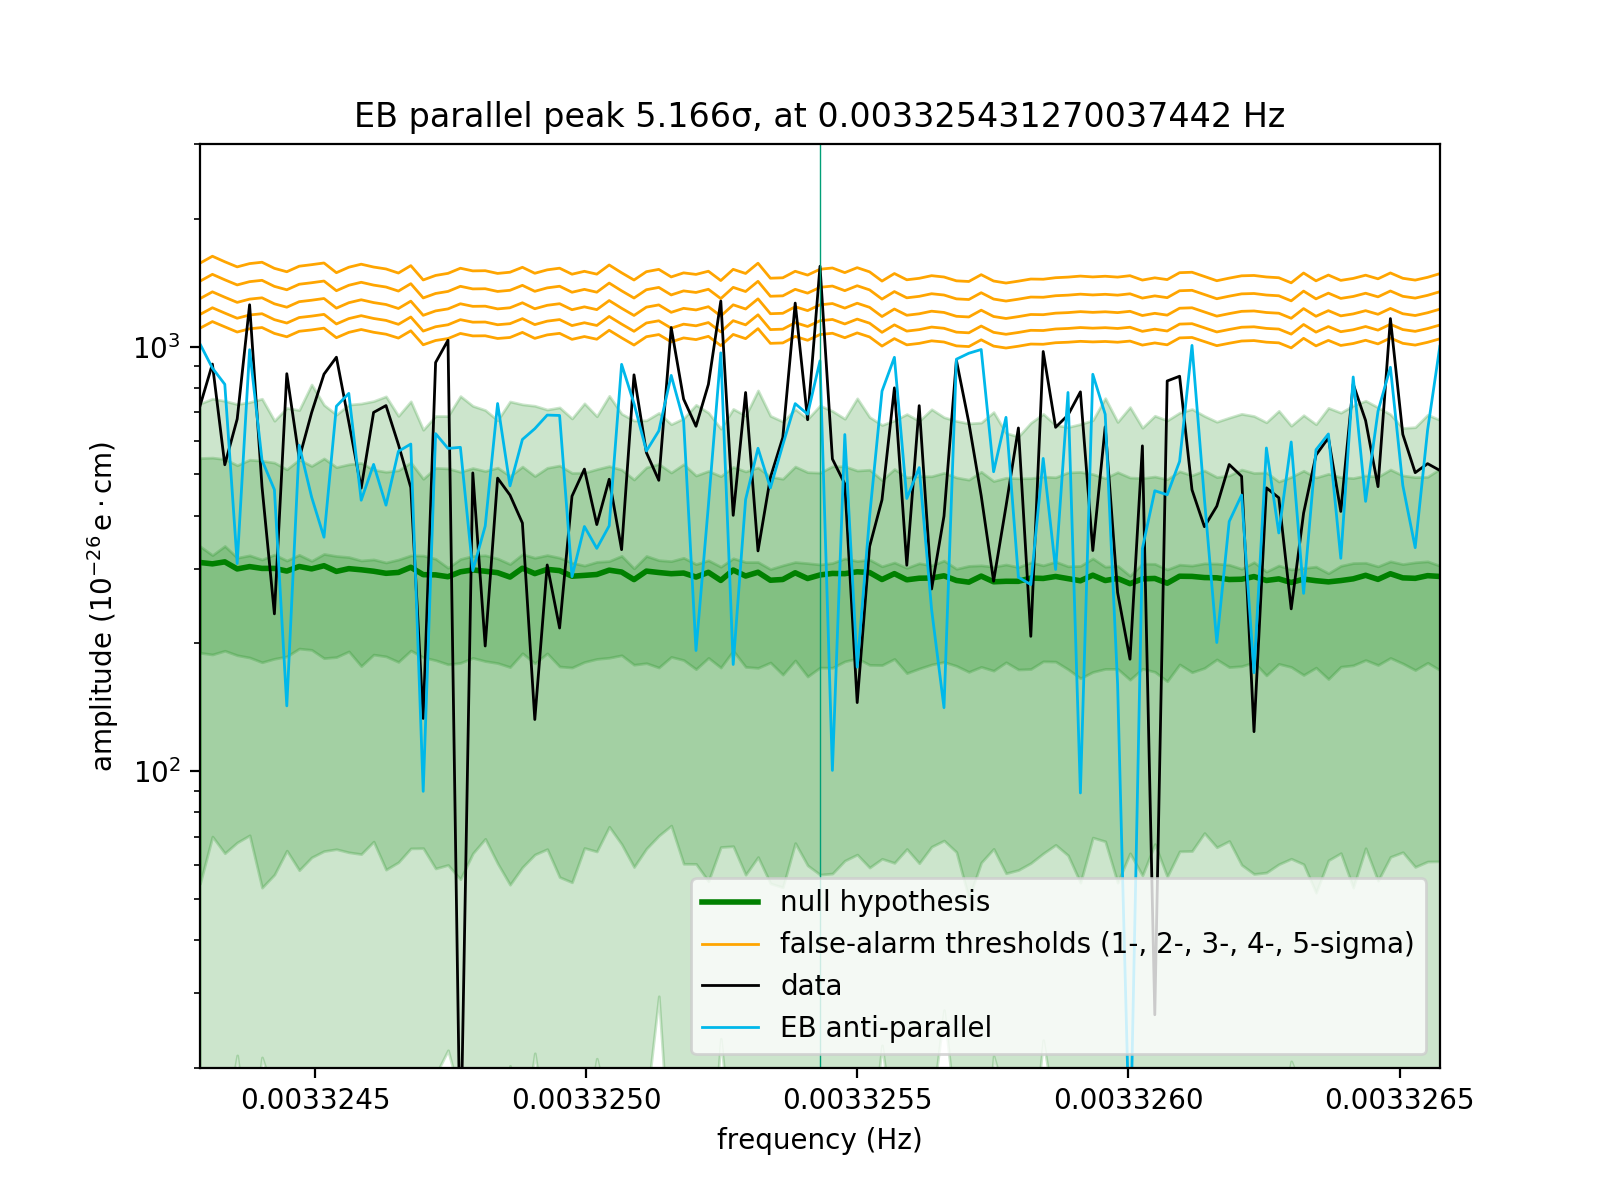
\includegraphics[width=\linewidth]{gfx/axions/P_detection_peak_145440.png}
  \caption{\ldots}
  \label{fig:P_detection_peak_145440}
\end{figure}


\section{E=0}

\begin{figure}
  \centering
  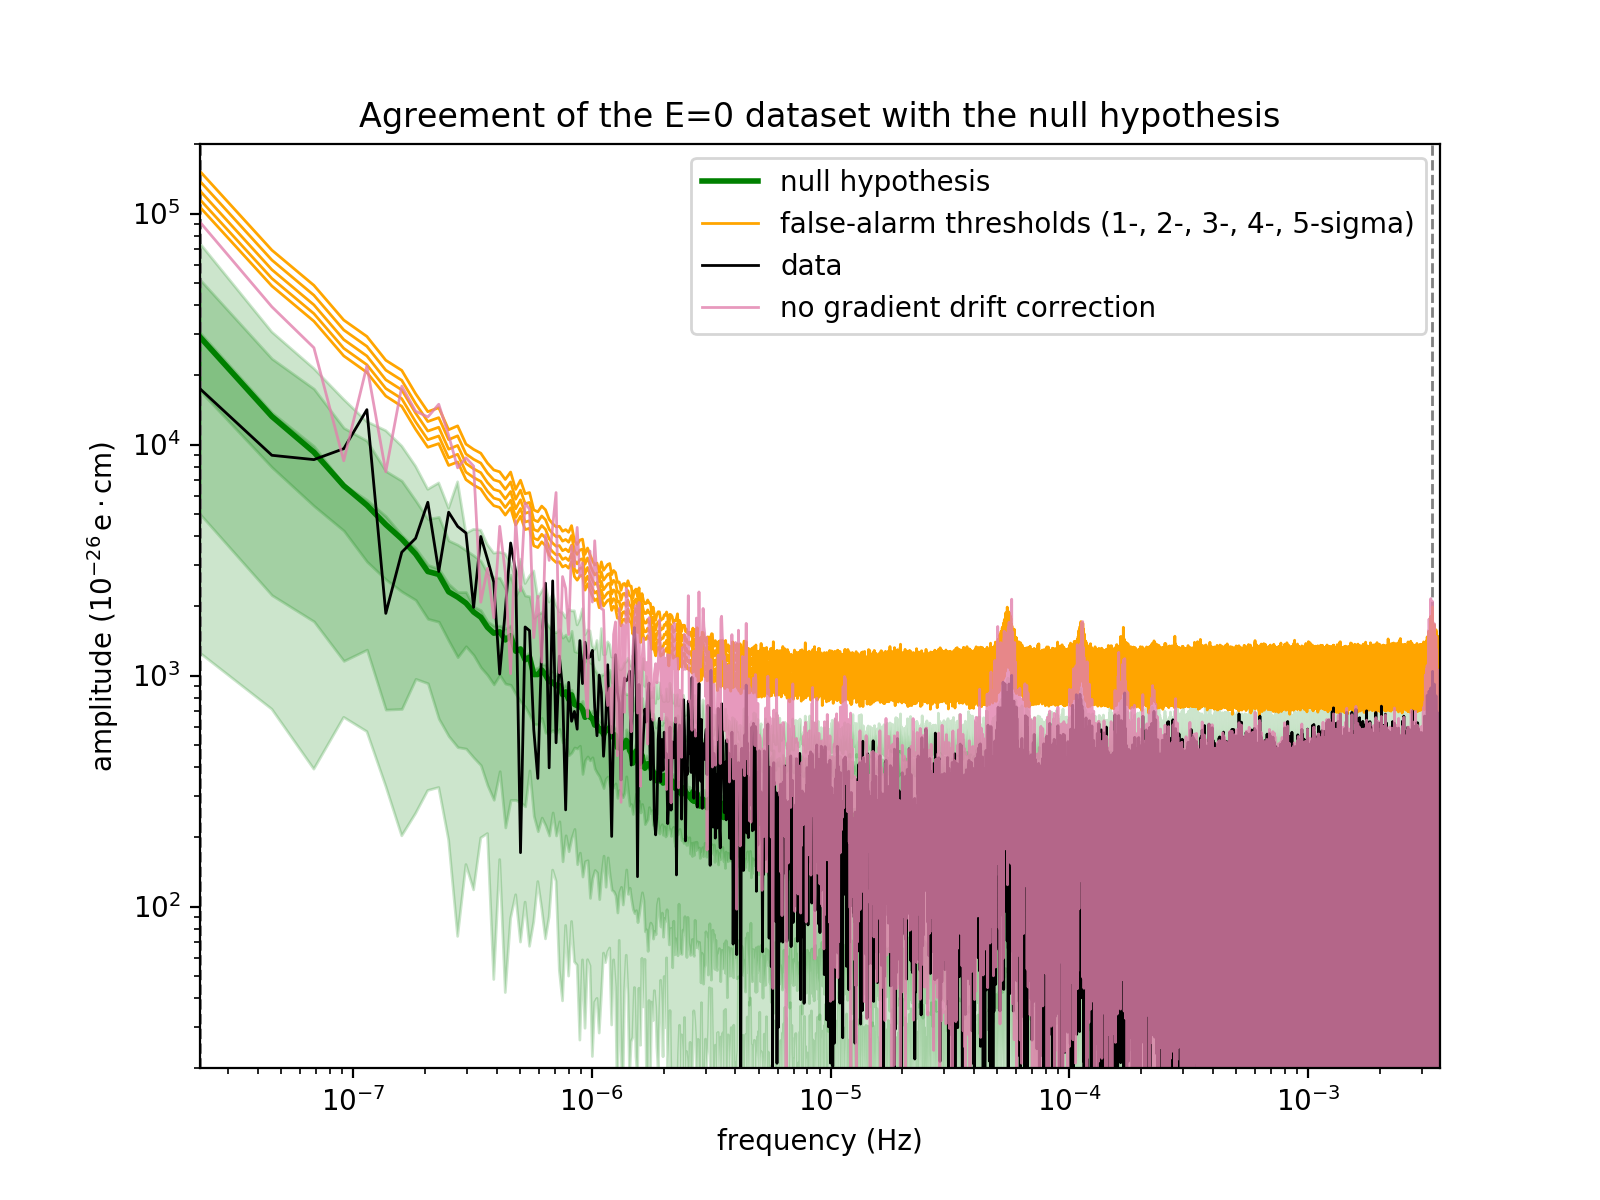
\includegraphics[width=\linewidth]{gfx/axions/E0_detection_and_no_GDC.png}
  \caption{\ldots}
  \label{fig:E0_detection_and_no_GDC}
\end{figure}
\begin{figure}
  \centering
  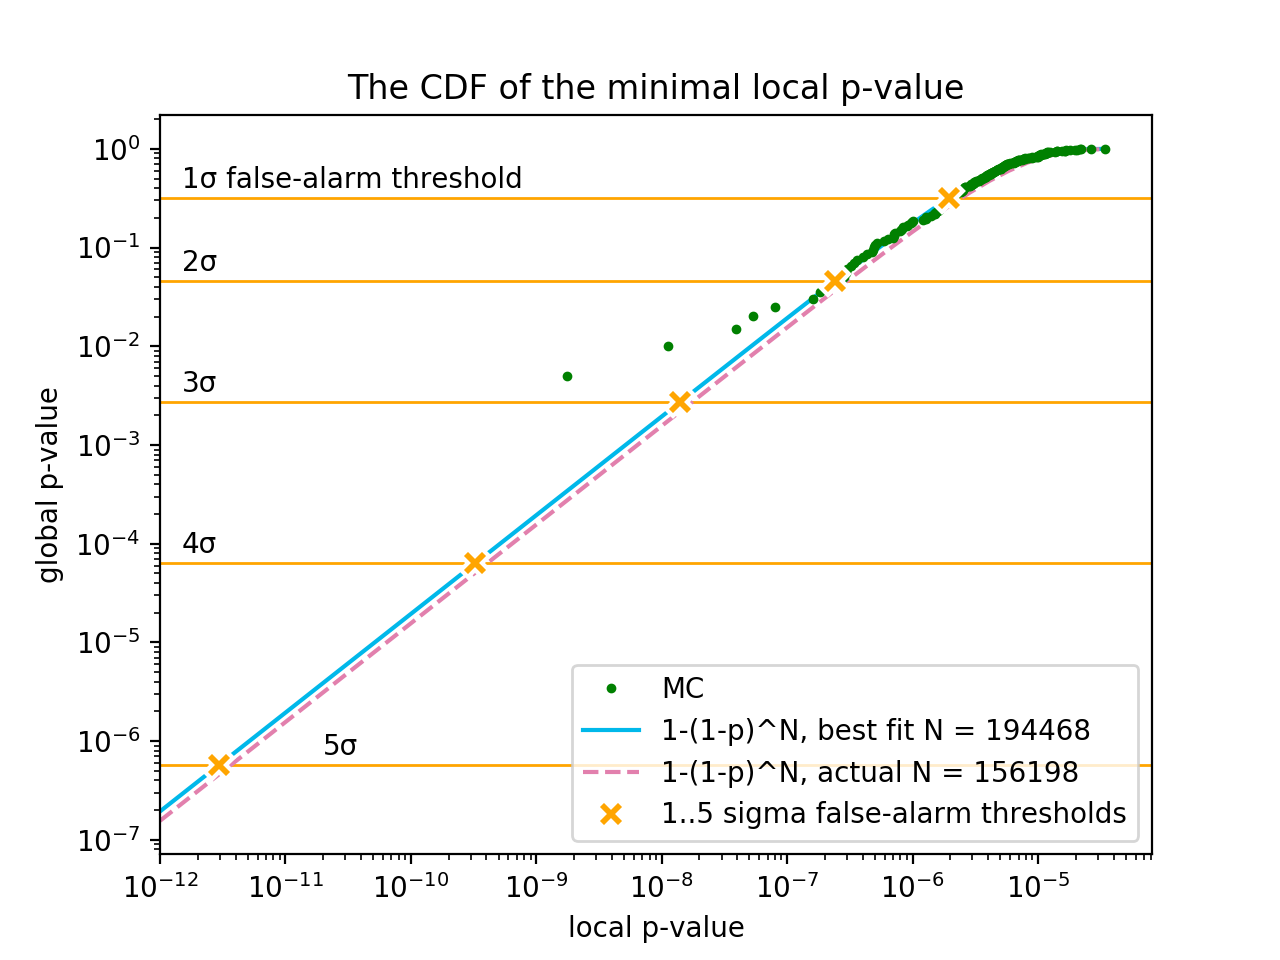
\includegraphics[width=\linewidth]{gfx/axions/E0_look-elsewhere.png}
  \caption{\ldots}
  \label{fig:E0_look-elsewhere}
\end{figure}
\begin{figure}
  \centering
  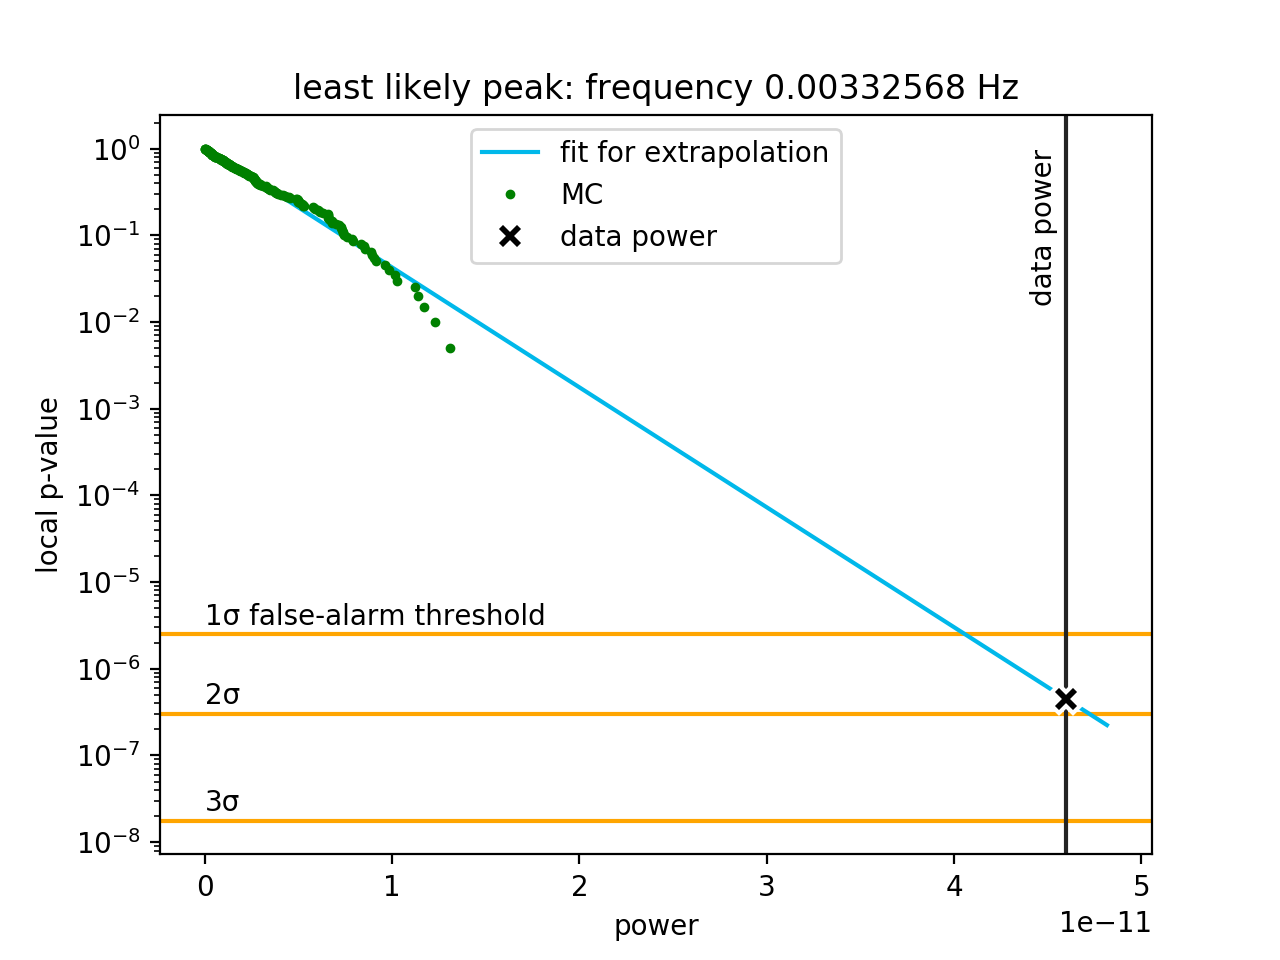
\includegraphics[width=\linewidth]{gfx/axions/E0_best_signal_candidate.png}
  \caption{\ldots}
  \label{fig:E0_best_signal_candidate}
\end{figure}



\chapter{Comparison of the analyses}